\documentclass{article}
\usepackage{multirow}
\usepackage{color,soul}
\usepackage{Sweave}
\begin{document}
\Sconcordance{concordance:draft1.tex:draft1.Rnw:%
1 2 1 1 0 4 1 1 8 59 1 1 11 13 1 1 8 17 1 1 8 299 1}


\makeatletter
\DeclareRobustCommand\bfseries{%
  \not@math@alphabet\bfseries\mathbf
  \fontseries\bfdefault\selectfont
  \boldmath % <-- added
}
\makeatother



\section*{Abstract} % fix the hazard ratios!!!! 

Community-driven online question and answer forums (CQA), platforms that allow users to ask and answer questions, contain an extensive amount of crowd-sourced information. One such example of a CQA is iFixit's \textit{Answers} forum. This forum features user-asked questions related specifically to device repair, which are answered by both repair experts and everyday users. An important aspect of these CQAs, for both users and the forum, is question response time. This paper presents a survival analysis of the time until a question receives it's first response. A Cox proportional hazards model was developed to predict the survival probability of a question, or the probability that a question receives an answer before a certain time. Though several predictors were signficant, the model's predictive accuracy was low ($R^2 = 0.15$). Significant predictors included the device category of the question (questions pertaining to Apple products received answers faster than others (HR...), factors related to the question's title (e.g., whether or not it was phrased as a question (HR..)), and the day of the week the question was posted (questions posted over the weekend received answers slower than those posted on a weekday (HR..)). Future studies can investigate whether factors identified as signifcant in this analysis can be generalized to other CQAs. 

%===================================================================================================
%===================================================================================================

\section*{1. Introduction}

Community-driven online question and answer forums have become widely-used sources of information. These online platforms feature thousands of user-posted questions and answers and receive millions of visits every month. The CQA analyzed in this paper is iFixit's \textit{Answers} forum. Founded in 2003, iFixit's mission is to equip users with the knowledge and tools necessary to repair their broken devices, as part of an effort to save money and reduce electronic waste. This company provides over 30,000 free online repair guides and sells specialized tools and parts needed for such repairs.
    
As not all possible repairs are covered in the published guides and users may have additional questions related to existing guides, iFixit's \textit{Answers} forum is an important resource for users. This platform features questions pertaining to over 9,000 devices, ranging from jammed zippers to shattered phone screens and faulty air conditioners, with over 100,000 user-posted solutions. As thousands of users rely on this forum for information, it is important that users receive timely answers. Fast response times have been shown to be associated with positive user satisfaction and, in turn, increase web traffic, which is valuable to the reputation and longevity of the CQA \cite{Rechavi2011}. Analysis of response times can reveal factors that affect how quickly questions receive answers, which can lead to suggestions for how users can ask better questions to minimize response times and for how the forum design can be improved.

However, analysis and prediction of response times on CQAs have not been thoroughly investigated. There is need for further analysis of response times in these forums, as the majority of existing research focuses on assessing and predicting question and answer quality. This paper presents a survival analysis on the time until a question receives its first answer on iFixit's \textit{Answers} forum, in order to determine factors significantly related to response time and to predict the survival probability of a question.

%===================================================================================================
%===================================================================================================

\section*{2. Related Work}
  
With the recent increase in the popularity and use of CQAs, these data-rich platforms have been the subject of a multitude of studies. Regarding analysis of response times, \cite{Bhat2014} developed a classification model using both textual and non-textual features to estimate response times for questions posted on \textit{Stack Overflow}. \cite{Mahmud2013} used parametric methods and proposed models to predict response times based on exponential distributions. \cite{Asaduzzaman2013} instead focused exclusively on unanswered questions and developed a taxonomy for classifying such questions and created a model to predict how long a question would remain unanswered. All research mentioned restricted analysis to either questions for which response times were observed or to questions that remained unanswered. The research presented in this paper uses survival analysis, a method not yet applied to CQAs, to allow for analysis of both answered and unanswered questions in a unified framework. 

The majority of existing research has been focused on predicting question and answer quality. \cite{Weimer2007} developed a classification algorithm to assess the quality of posts on \textit{Nabble.com} using primarily textual features of questions. \cite{Blumenstock} also determined that textual features (e.g. word count) was the most accurate predictor of Wikipedia article quality (Wikipedia articles can represent the same kind of user-generated content featured on CQAs). \cite{H.fu} instead found that non-textual features, like revision and comment count or the number of points a user has, were the most useful indicators of quality. A number of other studies have also developed classification algorithms using textual and non-textual features with the similar goal of predicting question or answer quality \cite{Yao2015} \cite{Toba2014} \cite{Ponzanelli2014a} \cite{Ravi2014}. The present analysis seeks to utilize both textual and non-textual features of questions on iFixit's \textit{Answers} forum to investigate if factors that indicate that a question is of high quality also lead to faster response times.

%===================================================================================================
%===================================================================================================

\section*{3. Materials}

% Table of derived predictors
\begin{table}[!htbp]
\centering
\begin{tabular}{| p{2cm} | p{10cm} |}
  \hline
  \multirow{9}{2cm}{Categorical Variables} & Device category the question pertains to. Categories include: Android/Other Phone, Apple Products, Camera, Electronics, Game Console, Home, Other, PC, Tablet, Vehicle \\ \cline{2-2}
  & If the question was posted on a weekend or on a weekday \\ \cline{2-2}
  & Whether or not the question's text contains any end punctuation marks (. ? !) \\ \cline{2-2}
  & Whether or not the question's text is in all lower case \\ \cline{2-2}
  & Whether or not the question's title contains at least one word considered to be ``frequently used'' among answered questions \\ \cline{2-2}
  & Whether or not the question's title contains at least one word considered to be ``frequently used'' among unanswered question \\ \cline{2-2}
  & Whether or not the question's title ends in a question mark \\ \cline{2-2}
  & Whether or not the user edited or added information to the question's text after posting it \\ \cline{2-2}
  & Whether or not the user made an effort to solve the problem prior to asking the question \\ \hline
  \multirow{5}{2cm}{Continuous Variables} & Average number of characters in each question's tags (Average tag length) \\ \cline{2-2}
  & Average frequency for all of a question's tags. Frequency defined as the proportion of times a tag appears in all of the data. Questions without tags were assigned a value of 0 (Average tag frequency) \\ \cline{2-2}
  & Number of characters in the question's text (Text length) \\ \cline{2-2}
  & Number of characters in the user-defined device name (Device name length) \\ \cline{2-2}
  & Ratio of the number of line breaks to the number of characters in the question's text (Line break to text length ratio) \\ \hline
\end{tabular}
\caption{Categorical and Continuous variables derived}
\label{table:variables}
\end{table}


The data analyzed contained 8,025 questions posted from April 8, 2017 to July 7, 2017 (date of data download). Variables in the data included: device name and category, title, text, tags, whether or not the user was a member of iFixit's site for less than one day before the question was posted, date and time the question was posted, and date and time the first answer was received. See Appendix for examples of answered and unanswered questions. Variables derived can be found in Table \ref{table:variables}. See Appendix for more details on variable derivation. 

%===================================================================================================
%===================================================================================================

\section*{4. Methods}

Questions analyzed were restricted to those posted in English. The time until event variable used in survival analysis was defined as the time since posting until a question received its first answer. For questions that did not receive an answer by the download date, time until event values were defined as the time since posting to the time the data was downloaded. Such questions were considered right-censored, meaning that exact answer times for these questions are greater than the observed download time (questions may receive answers after the download date) \cite{Kleinbaum2011}. 

Survival was defined as the event that a question did not receive an answer beyond a certain time, \textit{t}. Estimates of survival probability were generated with the Kaplan-Meier method, which adjusts to the presence of right-censored, or unanswered questions \cite{Bland1998}. From these estimates, survival curves were constructed to examine the survival experience of questions. Mean, median and other percentiles of survival times were also generated. 

As the probability distribution for response times is unknown, a nonparametric Cox proportional hazards model was developed to predict the survival probability of questions \cite{Moore2010}. To build the model, five-fold cross-validation was used \cite{Rodriguez2010}. Univariate analysis, performed on one training set, was used to identify variables to include in the final predictive Cox model \cite{Hammermeister1979}. Each predictor was entered into univariate Cox models and strength of association with response times was assessed. Those with partial likelihood ratio p-values of less than 0.001 were included in the final model.  Continuous predictors were entered into univariate Cox models both with and without square root and log transformations to determine the form of the predictor to include in the final model. Univariate analysis was again performed on each continuous predictor to investigate the use of splines. Each predictor, with the transformation found necessary in the previous analysis, was fit to three separate Cox models with restricted cubic splines of three, four, and five knots. AIC statistics were used to determine whether or not to include splines, as well as the optimum number of knots \cite{Harrell2015}. All predictors found to be signficant, along with transformations and splines found to be necessary, were included in the model for cross-validation. No variable selection was used after identifying significant predictors in univariate analysis, as \cite{Harrell2015} determined that reducing the number of predictors in the model decreased predictive accuracy more so than including all predictors. 

In each iteration of cross-validation, the full model was built on the training set and used to generate predicted hazard ratios on the corresponding test set. To assess prediction performance, predicted hazard ratios were entered into separate Cox models as the single quantitative predictor with response times as survival time. The resulting Nagelkerke's $R^2$ statistic, concordance statistic, Somers' \textit{Dxy}, partial likelihood ratio and p-value, were assessed as indicators of the model's performance \cite{Chen}. Signficant results from this model would indicate high predictive accuracy. The partial likelihood ratio assessed is a ratio of the log partial likelihood function evaluated at the parameter estimates, equivalent to a goodness of fit measure of the model with predictors, and the log partial likelihood function for the null model without predictors and only the baseline hazard function, equivalent to a goodness of fit measure for the null model. The p-value for this statistic was calculated from the $chi^2$ distribution \cite{Oakes1981}. Concordance statistics and Somers' \textit{Dxy} are a measure of the model's discriminative ability. Concordance is defined as the probability that for any two randomly chosen questions, the question with the shorter response time also has the higher predicted hazard. Concordance statistics close to 1 indicate high discriminative ability, while statistics close to 0.5 indicate discordance, or random predictions. Somers' \textit{Dxy} is the difference between the model's concordance statistic and discordance, 0.5. A Somers' \textit{Dxy} statistic of 0 indicates random predictions, while a statistic equal to 1 indicates perfect predictions \cite{Harrell2015}. These metrics were computed for each iteration on every training and test set. Averages of metrics across training and test sets were evaluated. The final model was then fit to the full data and the same metrics were computed and compared. 

Correlations between scaled Schoenfeld residuals, differences between observed and expected predictor values for questions that received answers, and a function of time, were examined to assess the proportional hazards assumption that the effect of predictors on hazard does not depend on time \cite{Grambsch1994}. Significant correlations would indicate a predictor has violated this assumption.

To compute predicted survival probabilities using the model, the \textit{predictSurvProb} function was used from the pec package in R. This function uses the Cox model and a vector of times to compute predicted survival probabilities. 

%===================================================================================================
%===================================================================================================

\section*{5. Results and Discussion}


% Distribution of answer times
\begin{figure}[!htbp]
  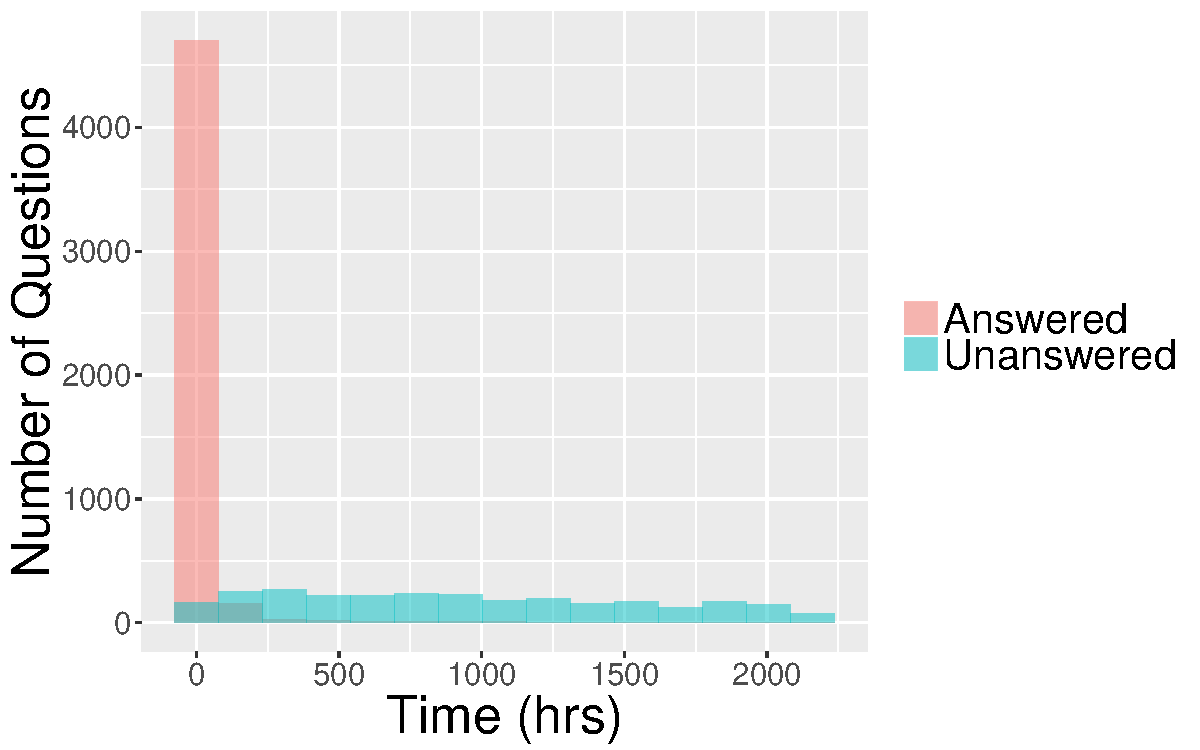
\includegraphics[scale=1]{times_dist.pdf}
  \caption{Distribution of response times}
  \label{fig:answertimes}
\end{figure}

% Kaplan-Meier curve
\begin{figure}[!htbp]
  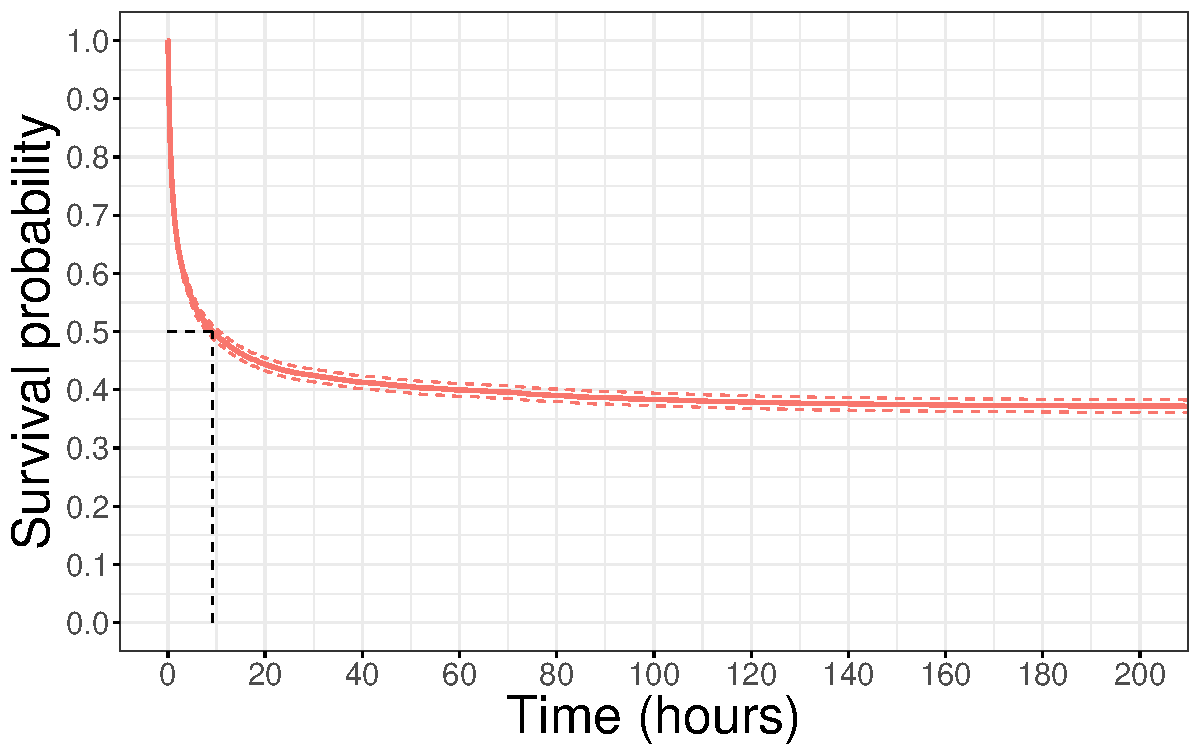
\includegraphics[scale=1]{kmcurve.pdf}
  \caption{Kaplan-Meier curve for all questions}
  \label{fig:kmcurve}
\end{figure}

  Of 8,025 questions in the full data, 7,760 were in English (97\% of the full data). Of those questions, 4,951 (63.8}\%) received an answer by the download date. The shortest response time was 0.5 hours. The longest was 2,159.02 hours (89.96 days). Figure ~\ref{fig:answertimes} shows the distribution of response times for all questions analyzed. 



  Figure ~\ref{fig:kmcurve} shows the Kaplan-Meier estimated survival probability curve for all questions in the data. The curve indicates that if a question does not receive an answer within the first 100 hours after it has been posted, the likelihood of it receiving an answer in the future is low. The Kaplan-Meier estimated mean survival time, or the average time until a question received its first answer was 775.75 hours, or 32.32 days. The median survival time, the time at which 50\% of the questions in the data received an answer, was 9.16 hours.

% % Univariate analysis results
% \begin{table}[!htbp]
% \centering
% \begin{tabular}{| p{5cm} | p{2.75cm} | p{2cm} |}
%   \hline
%   \textbf{Continuous Predictors} & \textbf{Transformation} & \textbf{p-value} \\ 
%   \hline \hline
%   \multirow{ 3 }{ 5cm }{ Average tag frequency }
%   & Untransformed & 1.270620e-08 \\
%   & Log + 1 & 1.186521e-08 \\
%   & \textbf{*}Square root & 1.464184e-11 \\ \hline
%   \multirow{ 3 }{ 5cm }{ Average tag length }
%   & Untransformed & 2.611529e-02 \\ 
%   & \textbf{*}Log + 1 & 6.018542e-05 \\
%   & Square root & 2.999917e-04 \\ \hline
%   \multirow{ 3 }{ 5cm }{ Device name length }
%   & Untransformed & 6.530431e-03 \\
%   & \textbf{*}Log + 1 & 1.912977e-05 \\
%   & Square root & 2.291424e-04 \\ \hline
%   \multirow{ 3 }{ 5cm }{ Line break to text length ratio } 
%   & Untransformed & 1.398819e-07 \\
%   & Log + 1 & 1.092952e-07 \\
%   & \textbf{*}Square root & 1.148792e-11 \\ \hline
%   \multirow{ 3 }{ 5cm }{ Text length }
%   & Untransformed & 6.947221e-12 \\
%   & \textbf{*}Log & 0.000000e+00 \\
%   & Square root & 1.110223e-16 \\ \hline \hline
%   \multicolumn{ 2 }{ |l| }{ \textbf{ Categorical Predictors } } & \textbf{ p-value } \\ \hline \hline
%   \multicolumn{ 2 }{ |l| }{ \textbf{*}Device category } & 0.000000e+00 \\ \hline
%   \multicolumn{ 2 }{ |l| }{ \textbf{*}Weekend or Weekday } & 4.123729e-04 \\ \hline
%   \multicolumn{ 2 }{ |p{7.75cm}| }{ \textbf{*}Whether or not the question's text contained at least one end punctuation mark } & 2.535394e-09 \\ \hline
%   \multicolumn{2}{ |p{7.75cm}| }{ \textbf{*}Whether or not the question's text is in all lower case } & 1.540030e-07 \\ \hline
%   \multicolumn{2}{ |p{7.75cm}| }{ \textbf{*}Whether or not the question's title contains terms considered to be frequently used among answered questions } & 7.639738e-05 \\ \hline
%   \multicolumn{2}{ |p{7.75cm}| }{ \textbf{*}Whether or not the question's title contains terms considered to be frequently used among unanswered questions } & 0.000000e+00 \\ \hline
%   \multicolumn{2}{ |p{7.75cm}| }{ \textbf{*}Whether or not the question's title ended in a questionmark } & 1.142308e-12 \\ \hline
%   \multicolumn{2}{ |p{7.75cm}| }{ \textbf{*}Whether or not the user edited or added information to the question's text sometime after posting it } & 2.547222e-07 \\ \hline
%   \multicolumn{2}{ |p{7.75cm}| }{ \textbf{*}Whether or not the user had been a member for less than one day before the question was posted } & 0.000000e+00 \\ \hline
%   \multicolumn{2}{ |p{7.75cm}| }{ \textbf{*}Whether or not the user made an effort to solve the problem on their own, prior to asking the question } & 3.164815e-05 \\ \hline
% \end{tabular}
% \caption{Univariate analysis results} 
% \label{table:univariate_results}
% \end{table}


Each training set contained 6,208 questions, and each test set contained 1,552 questions. Univariate analysis performed on one training set indicated that all cateogorical predictors were signficant with partial likelihood ratio p-values of less than 0.001. All continuous predictors, except for device length and average tag length, also resulted in univariate p-values of less than 0.001. Applying either square root or log transformations to continuous variables resulted in univariate p-values of less than 0.001. For continuous predictors that contained zeros, one was added to each observation before applying the log transformation. The following transformations were applied to continuous variables: square root transformation of average tag frequency, log plus 1 transformation of average tag length, log plus 1 transformation of device name length, square root transformation of line break to text length ratio, and log transformation of text length. All categorical predictors and all continuous predictors with necessary transformations were retained for the full model. 

% Splines
\begin{table}[!htbp]
\centering
\begin{tabular}{| p{5cm} | l | l |}
  \hline
  \textbf{Predictor} & \textbf{K} & \textbf{AIC} \\ 
  \hline
  \multirow{ 4 }{ 5cm }{ Log transformation of text length } 
  & 0 & 65862.83 \\ 
  & \textbf{*}5 & 65862.02 \\ 
  & 4 & 65863.35 \\ 
  & 3 & 65862.08 \\ 
  \hline
  \multirow{ 4 }{ 5 cm }{ Square root transformation of line breaks to text length ratio }
  & 0 & 65890.28 \\ 
  & 5 & 65884.70 \\ 
  & 4 & 65882.98 \\ 
  & \textbf{*}3 & 65881.93 \\ 
  \hline
  \multirow{ 4 }{ 5 cm }{ Square root transformation of the average tag frequency }
  & \textbf{*}0 & 65890.75 \\ 
  & 5 & 65891.69 \\ 
  & 4 & 65891.75 \\ 
  & 3 & 65892.35 \\ 
  \hline
  \multirow{ 4 }{ 5 cm }{ Log transformation of device name length + 1 }
  & 0 & 65918.06 \\ 
  & \textbf{*}5 & 65847.34 \\ 
  & 4 & 65880.89 \\ 
  & 3 & 65898.00 \\ 
  \hline
  \multirow{ 4 }{ 5 cm }{ Log transformation of average tag length + 1 }
  & 0 & 65920.24 \\ 
  & 5 & 65911.20 \\ 
  & \textbf{*}4 & 65910.81 \\ 
  & 3 & 65914.98 \\ 
   \hline
\end{tabular}
\caption{Determining the optimal k number of splines for each predictor} 
\label{table:splines}
\end{table}

Table \ref{table:splines} shows the results of determining the optimal number of knots for each continuous predictor. Those marked with an asterisk (*) were included in the final model. 

% Cross-validation metrics
\begin{table}[!htbp]
\centering
\begin{tabular}{| r | r | r | r | r  | r | r | r |}
  \hline
 & \textbf{HR} & \textbf{LR} & \textbf{p-value} & \textbf{$R^2$} & \textbf{\textit{Dxy}} & \textbf{Concordance} \\ 
  \hline
  \textbf{Training Sets} & 2.027030 & 937.3877 & 0.0000 & 0.1401511 & 0.2683734 & 0.6341867 \\ 
  \textbf{Test Sets} & 1.986844 & 220.8309 & 0.0000 & 0.1400518 & 0.2582790 & 0.6291395 \\
  \textbf{Full Data} & 2.028051 & 1165.0321 & 0.0000 & 0.1394092 & 0.2672884 & 0.6336442 \\ 
   \hline
\end{tabular}
\caption{Performance Metrics. HR: Hazard Ratio, LR: Partial Likelihood Ratio} 
\label{table:cv}
\end{table}

Average performance metrics for test and training sets are in Table \ref{table:cv}. Partial likelihood ratios and p-values indicate that the model as a whole is signficantly associated with response time. However, $R^2$ statistics and discrimination indexes are considerably low. Metrics for the final model's performance on the full data, also found in Table \ref{table:cv}, are consistent with metrics found in cross-validation and indicate low predictive accuracy. Results for training, test, and the full data did not change significantly, indicating that the model was not overfit. 

% Final model on full data
\begin{table}[!htbp]
\centering
\begin{tabular}{|p{3cm} p{4cm}| c | c |}
  \hline
 \textbf{Variable} & & \textbf{Coefficient (SE)} & \textbf{p-value} \\ \hline
  \multirow{ 9 }{ 3 cm }{ Device Category } & Apple Product & 0.9346 (0.0476) & <0.0001 \\ 
  & Camera & -0.3199 (0.0476) & \\ 
  & Electronics & -0.0138 (0.0904)  & \\ 
  & Game Console & 0.2458 (0.0784)  & \\ 
  & Home & 0.3368 (0.0697) &  \\ 
  & Other & -0.1304 (0.0555)  & \\ 
  & PC & 0.2818 (0.0597) &  \\ 
  & Tablet & -0.1566 (0.0815)  & \\ 
  & Vehicle & 0.4056 (0.0695)  & \\ 
  \hline
  \multicolumn{ 2 }{ |l| }{ Weekend or weekday } & -0.1334 (0.0331)  & <0.0001 \\ \hline
  \multicolumn{ 2 }{ |p{7.5cm}| }{ Whether or not the question's text contained at least one end punctuation mark } & 0.0247 (0.0499) & 0.6127 \\ \hline
  \multicolumn{ 2 }{ |p{7.5cm}| }{ Whether or not the question's text is in all lower case } & -0.1770 (0.0645) &  0.0060 \\ \hline
  \multicolumn{ 2 }{ |p{7.5cm}| }{ Whether or not the question's title contains terms considered to be frequently used among answered questions } & 0.0475 (0.0422) &  0.2596 \\ \hline
  \multicolumn{ 2 }{ |p{7.5cm}| }{ Whether or not the question's title contains terms considered to be frequently used among unanswered questions } & -0.2808 (0.0340)  & <0.0001 \\ \hline
  \multicolumn{ 2 }{ |p{7.5cm}| }{ Whether or not the question's title ended in a questionmark } & 0.2571 (0.0332) &  <0.0001 \\ \hline
  \multicolumn{ 2 }{ |p{7.5cm}| }{ Whether or not the user edited or added information to the question's text sometime after posting it } & 0.2983 (0.0857)  & 0.0005 \\ \hline
  \multicolumn{ 2 }{ |p{7.5cm}| }{ Whether or not the user had been a member for less than one day before the question was posted } & -0.1069 (0.0364)  & 0.0031 \\ \hline
  \multicolumn{ 2 }{ |p{7.5cm}| }{ Whether or not the user made an effort to solve the problem on their own, prior to asking the question } & -0.0724 (0.0362)  & 0.0448 \\ \hline
  \multicolumn{ 2 }{ |p{7.5cm}| }{ Square root of the average tag frequency } & 2.2609 (0.7196)  & 0.0020 \\ \hline
\end{tabular} 
\caption{Coefficients for predictors in the final model.Continous predictors with restricted cubic splines are not shown. } 
\label{table:coefficients}
\end{table}

% Final model statistics
\begin{table}[!htbp]
\centering
\begin{tabular}{| r | r |}
  \hline
  \textbf{LR} & 1265.291 \\ \hline
  \textbf{p-value} & 0 \\ \hline
  \textbf{$R^2$} & 0.150 \\ \hline
  \textbf{\textit{Dxy}} & 0.267 \\ \hline
\end{tabular}
\caption{Final model statistics} 
\label{table:final model}
\end{table}

Assessing the proportional hazards assumption indicated that several levels of the device categorization variable, specifically Apple Product, Camera, Game Console, and Other, violated the assumption. 

Interpretations of the coefficients highlighted in Table \ref{table:coefficients}:

\begin{itemize}
  \item The estimated hazard of receiving an answer is 154.1\% (95\% CI (131.5\%, 180.0\%)) higher for questions pertaining to Apple products than the hazard for questions about Android and Other phones, controlling for all other predictors.
  \item The estimated hazard of receiving an answer for questions posted on a weekend is 12.5\% (95\% CI (6.7\%, 18.0\%)) lower than the hazard for questions posted on a weekday, controlling for all other predictors.
  \item The estimated hazard of receiving an answer is 24.5\% (95\% CI (19.3\%, 29.4\%)) lower for questions with titles that contain at least one word considered to be frequently-used among unanswered questions, than the hazard for questions with titles that do not, controlling for all other predictors. 
\end{itemize}

See Table \ref{table:coefficients} for the full list of model coefficients. Table \ref{table:final model} displays statistics for the final model. 

Results and coefficients of the final model reveal how users can ask questions in order to decrease response time. Findings suggest that users should phrase the title in the form of a question, use correct grammar (e.g. punctuation and capitalization), include specific and concise tags, and post the question on a weekday. 

The model's weak predictive accuracy, which may be explained by limitations in the data, lead to suggestions for changes in CQA design. Many users asking a question incorrectly specified the device name (e.g. A user asking a question about a Turtle Beach Ear Force XO ONE headset defined the device name as, ``Turtle Beach Ear Force Xmy grandson chewed through the wire while he was playing it's brand-new is there anyway I can have it fixed0 One''), or did not include a device name at all. Many users also incorrectly used the tagging system by including ambiguous and lengthy tags like ``someone sat on it :('' or ``help me please!!!!!'' (tags are generally a couple key words that allow the answering community to quickly discern the question's topic). It is likely that these inconsistencies contributed to the final model's low predictive power. This, along with the results of the final model, reveal some of the ways that the CQA can be structured to improve analysis and decrease response time. As findings indicate that questions with correctly defined tags and device names may lead to quicker response times, the CQA can provide a stricter framework for asking questions. Allowing users to enter any device name or tag leaves room for user error, shown by the examples described above. Instead, the CQA can restrict the tags or devices that users can include to a drop-down list. The CQA can also include more tips to guide users asking questions. Establishing and implementing a more restrictive framework for asking questions can help users ask understandable and clear questions and in turn decrease response time, as well as create a set of consistent questions for improved analysis. 

%===================================================================================================
%===================================================================================================

\section*{6. Conclusion}

This study developed a Cox proportional hazards model to predict the probability that a question posted on iFixit's \textit{Answers} forum receives an answer before a certain time. Predictors found to be signficant included: device category, if the question was posted on a weekend or a weekday, whether or not the question's text contained at least one word considered frequently-used among unanswered questions, and whether or not the question's title ends in a questionmark. While overall the model was signficant, its predictive performance was considerably low. 

%===================================================================================================
%===================================================================================================

\section*{7. Acknowledgement}

This research was supported by the Bill and Linda Frost fund of the California Polytechnic State University of San Luis Obispo. Special thanks goes to iFixit for providing access to the CQA data and for the help and assistance in its analysis. 

%===================================================================================================
%===================================================================================================

\section*{8. Appendix} 

% --------------------------------------------------------------------------------------------------
\subsection*{8.1 Posted questions}

% answered question id = 397414
% unanswered question id = 399971
% Table to display questions
\begin{table}[!htbp]
\centering
\begin{tabular}{| l | l | p{6cm} | l |}
  \hline
 \textbf{Answered} & \textbf{Device} & \textbf{Title} & \textbf{Date Posted} \\
  \hline
  Yes & iPhone 6 & iPhone water damage, touch screen issue &  2017-05-10 21:50:48 GMT \\ \cline{2 - 4}
  & \textbf{New User} & \textbf{Text} & \textbf{Date of First Answer} \\ \cline{2 - 4}
  & Yes & So I dropped my iPhone in water 4 days ago. Have done the whole rice thing and seen huge difference in it. However, only one side of my screen works and it is the one side which I need to unlock the phone. What would be the best way forward? & 2017-05-10 23:12:27 GMT \\ \cline{4 - 4}
  & & & \textbf{Response Time (hr)} \\ \cline{4 - 4}
  & & & 1.361 \\ \cline{4-4} \hline \hline
  \textbf{Answered} & \textbf{Device} & \textbf{Title} & \textbf{Date Posted} \\ \cline{1 - 4}
  No & android tablet & ccccaaaan you help me fix my touch screen & 2017-05-23 07:35:12 GMT \\ \cline{2 - 4}
  & \textbf{New User} & \textbf{Text} & \textbf{Date of First Answer} \\ \cline{2 - 4}
  & No & touch screen not worki & NA \\ \cline{4 - 4}
  & & & \textbf{Response Time (hr)} \\ \cline{4 - 4}
  & & & NA \\ 
   \hline
\end{tabular}
\caption{Answered and unanswered questions}
\label{table:questions}
\end{table}

Table \ref{table:questions} provides an example of an answered and unanswered question. All fields in the table are shown as the users entered it. 

% ------------------------------------------------------------------------------------------------

\subsection*{8.2 Variable Derivation}

\subsubsection*{8.2.1 Device Categorization}

Original device categories defined by iFixit included: Apparel, Appliance, Camera, Car and Truck, Computer Hardware, Electronics, Game Console, Household, Mac, Media Player, PC, Phone, Skills, Tablet, Vehicle. Device titles were parsed and certain categories were combined or separated to create a new device categorization variable to use in the Cox model. Final categories created included: Android/Other Phone, Apple Product, Camera, Electronics, Game Console, Home, Other, PC, Tablet, Vehicle. Under the original device categorization, 1,954 questions (25.2\% of 7,760) were categorized incorrectly and indicated an NA for its category. Missing values were a result of users creating questions for devices not already in the iFixit's database, or from the user incorrectly defining the device name. For questions with missing categories, key words were searched for in device titles to recategorize accordingly. All other questions with ambiguous device titles were categorized as Other. 

% ------------------------------------------------------------------------

\subsubsection*{8.2.2 Whether or not the question's text contained at least one end punctuation mark}

This variable was created to investigate if run-on sentences, sentences with no end punctuation, take longer to receive an answer.

% ------------------------------------------------------------------------

\subsubsection*{8.2.3 Whether or not the question's title contains terms considered to by frequently-used among answered/unanswered questions}

These variables were created to investigate if questions pertaining to popular topics receive answers faster than questions that do not. Similarly, another variable was created to investigate if questions pertaining to unpopular topics receive answers slower than qustions that do not. This variable was created based off of methods from \cite{Correa2013} and \cite{Ravi2014}.

To create the variables, the data was separated between answered and unanswered questions. For the data frame containing answered questions, text mining techniques were used to create a list of every word within each questions' titles and the proportion of times those words occurred among all answered questions' titles, defined as the frequency. The same was performed for the data frame containing unanswered questions. ``Frequently-used'' words in answered questions were defined as those that appeared in 1\% or more of all answered questions' titles, and appeared in more answered questions than in unanswered questions. To determine the latter, a ratio of frequencies was assessed. The ratio was calculated as the proportion of times a word occured among answered questions, to the proportion of times a word occured in unanswered questions. As an example, if ``cracked'' appeared in 2\% of answered questions and 0.1\% of unanswered questions, it would be considered ``frequently-used'' among answered questions as it occurs in more than 1\% of answered questions' titles and occurs 20 times more in answered question than in unanswered questions (ratio = 0.02/0.001 = 20). Similarly, ``frequently-used'' words in unanswered questions must occur in 1\% or more of all unanswered question's titles and occur in more unanswered questions than answered questions. As there was some overlap between ``frequently-used'' words in each list and levels of the device categorization variable, every word that matched a device name was removed from the lists. The resulting list for answered questions contained 111 words. The list for unanswered questions contained 32 words. Lists can be found in Table \ref{table:frequent_terms}

% Table with list of frequently used words
\begin{table}[!htbp]
\centering
\begin{tabular}{|p{4cm}|p{8cm}|}
  \hline
 \textbf{Frequently-used terms among answered questions} & screen, turn, working, replacement, power, work, replace, charging, charge, button, touch, black, turning, broken, start, stuck, new, lcd, upgrade, problem, change, port, replaced, card, open, boot, replacing, remove, reset, back, drive, error, cable, ssd, cracked, hard, one, dropped, logic, lines, white, keeps, pro, dead, now, front, damage, switch, parts, glass, still, charger, issue, sim, turns, digitizer, just, mode, model, backlight, usb, stopped, logo, starting, know, unresponsive, password, factory, call, use, damaged, find, sensor, possible, fixed, side, galaxy, data, ipod, problems, issue, slow, system, connector, without, overheating, code, ram, air, microphone, please, red, much, plugged, getting, booting, left, way, buy, plus, time, loose, lock, coming, got, shuts, says, install, key, door, top \\
  \hline
  \textbf{Frequently-used terms among unanswered questions} & sound, light, wifi, speaker, connect, picture, stay, noise, bluetooth, isnt, apps, going, rear, question, play, stop, service, take, hear, lights, showing, network, volume, come, keep, connection, flashing, shut, print, blue, buttons, edit \\ 
   \hline
\end{tabular}
\caption{Frequently-used terms among answered and unanswered questions' titles, ordered by decreasing frequency}
\label{table:frequent_terms}
\end{table}

% ------------------------------------------------------------------------

\subsubsection*{8.2.4 Whether or not the question's title ended in a question mark}

This variable was created to investigate if questions with titles in the form of questions receive answers faster than those that do not \cite{Bhat2014}. 

% ------------------------------------------------------------------------

\subsubsection*{8.2.5 Whether or not the user made an effort to solve the problem on their own, prior to asking the question}

Logical variable indicating true if the asker included words in the question's text that indicate that prior effort was made to find the solution to the question before posting. Words searched for include: tried, searched, researched, tested, replaced, used, checked, investigated, considered, measured, attempted, inspected, fitted. This variable was created based off of findings and methods from \cite{Bhat2014} \cite{Harper2008}. 

% ------------------------------------------------------------------------

\subsubsection*{8.2.6 Average tag frequency}

This variable was created to investigate if including popular or widely-used tags in a question lead to faster response times. This variable is the average frequency, or proportion of times a question's tags appear in all of the data set. If a question has a higher average, than at least one of it's tags are frequently used. This variable was created based off of findings from \cite{Bhat2014}. 

% ------------------------------------------------------------------------

\subsubsection*{8.2.7 Average tag length}

This variable was created to investigate if questions with correctly defined tags have faster response times than questions that do not include tags or incorrectly use the tagging system. It is hypothesized that questions with ambiguous or lengthy tags make it difficult for the answering community to discern the question's topic, and thus have slower response times or remain unanswered. 

% ------------------------------------------------------------------------

\subsubsection*{8.2.8 Device name length}

This variable was created to investigate if questions with correctly defind device names have faster response times than questions that do not include a name or are incorrectly defined. Similar to the average tag length variable, it is hypothesized that questions with incorrectly defined device names make it difficult for the answering community to discern the question's topic, and thus have slower response times. 

% ------------------------------------------------------------------------

\subsubsection*{8.2.9 Line break to text length ratio}

This variable was created to investigate if questions that include line breaks in the text are easier to read than questions that don't include any, and thus have shorter response times. 

% ------------------------------------------------------------------------



\bibliography{questions}
\bibliographystyle{ECA_jasa}









\end{document}
